\documentclass{article}

\usepackage{hyperref}
\usepackage{amsmath}
\usepackage{amsfonts}
\usepackage{amssymb}
\usepackage{graphicx}

\title{Introduction to Quantum Information and Computing - Lecture 1}
\author{Shrikara A, Arnav Negi, Kriti Gupta, Manav Shah, Mohammed Shamil,\\ Shiven Sinha, Swayam Agarwal, Vineeth Bhat, Yash Adivarekar} % add contributors
\date{3rd January, 2023}

\begin{document}


    \pagenumbering{gobble}
    \maketitle
    \vfill
    \tableofcontents
    \newpage
    \pagenumbering{arabic}


    %fill
    \section{Introduction and Motivation}
        \subsection{Introduction}

            Quantum mechanics is a fundamental theory in physics that provides a description of the physical properties of nature at the scale of atoms and subatomic particles. It is a superset of classical mechanics and can explain
            behaviour in experiments that are not explained by only classical mechanics laws. One such experiment is
            the Stern Gerlach experiment.\\

            The mathematical framework for quantum mechanics is linear algebra. States are described as vectors in a complex
            vector space, while measurements and operators are linear operators that act on the space.\\
            
            
        \subsection{Stern-Gerlach Experiment}

            Silver atoms are heated in an oven and projected at a screen through a hole. The stream of silver atoms 
            are subjected to a homogeneous magnetic field. This causes them to bend in trajectory upwards or downwards.\\

            The magnetic moment of the atom is proportional to the spin of the atom's unpaired electron: $\mu \propto S$\\
            
            Because the interaction energy of the magnetic moment with the magnetic field
            is just $-\mu \cdot B$ , the z-component of the force experienced by the atom is given by,
            $$\textbf{F}_z = \frac{\partial}{\partial z}(-\mu \cdot B) \simeq \mu_z\frac{\partial B_z}{\partial z}$$
            The expected pattern is that of a band of silver, however only two spots are observed. This implies
            the spin of the atoms along the Z-axis is quantized to two values, $S_z+$ and $S_z-$. This goes against the classical prediction.

            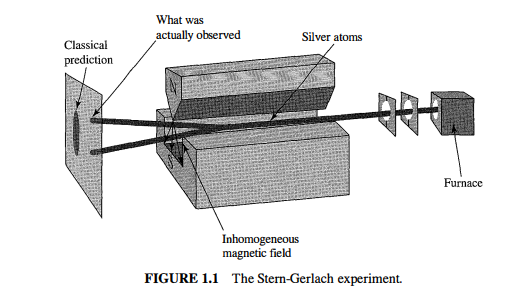
\includegraphics[width = 12 cm]{sterngerlach.png}

            Moreover, on sequential Stern-Gerlach experiments, more non classical behaviour was seen.\\

            In the experiment, $S_z$ was measured and the atoms with $S_z-$ spin are blocked. Then the rest are
            sent through another Stern-Gerlach for measuring $S_x$. Again, the atoms with spin $S_x-$ are blocked.
            The final leftover atoms are passed through an experiment measuring $S_z$ again. \\

            It is found that even though all atoms with $S_z-$ were blocked, there still are atoms with $S_z-$ spin
            after the third experiment. This phenomenon cannot be explained by classical mechanics. Measuring $S_x$ destroys any information obtained about the $S_z$ component of the atoms.

            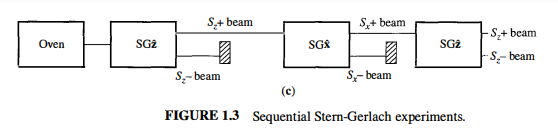
\includegraphics[width = 12 cm]{seqSG.png}
            
        \subsection{Shannon's Theory of Information and Entropy}
            Claude Shannon created the modern information theory. He justified use of entropy as measure of information
            about a system. The units for information were taken as bits. In terms of quantum information, the units are 
            qubits. \\

            Shannon defined entropy as the average measure of randomness or uncertainty in a system. The Shannon entropy 
            is defined as entropy H (Greek capital letter eta) of a discrete random variable $X$, which takes values in the alphabet $\mathcal{X}$ and is distributed according to \\
            
            $$p : \mathcal{X} \longrightarrow [0,1]$$ such that $$p(x) := \mathbb{P}[X = x]$$

            And H is given by \\
            $$H(\mathcal{X}) = \mathbb{E}[-logp(X)] = -\sum_{x \in \mathbb{X}}p(x)logp(x)$$
            

        \subsection{No Cloning Theorem}

            In physics, the no-cloning theorem states that it is impossible to create an independent and identical copy of an arbitrary unknown quantum state. This has profound implications in quantum computation. The theorem follows from the fact that all quantum operations must be unitary linear transformation on the state.

        \subsection{Outline of the Course}
            In the course we will be exploring the following topics:
            
            \begin{enumerate}
                \item Postulates
                \item Everything is a quantum channel
                \item Entanglement, Separability, Non-locality
                \item Teleportation, No Cloning
                \item Entropy, Trace Distance
            \end{enumerate}


    \section{Finite Dimensional Hilbert Spaces}
        A \textit{d}-dimensional Hilbert space $\mathcal{H}$ ($1 \leq d < \infty$) is a complex vector space with an inner product defined on it. A vector in the Hilbert space $\mathcal{H}$ is denoted by $|\psi\rangle $. The inner product $\langle . ,. \rangle : \mathcal{H} \times \mathcal{H} \rightarrow \mathbb{C} $ has the following properties:
        \begin{itemize}
            \item \textit{Non negativity -} $\langle \psi , \psi \rangle \geq 0$ $\forall$ $|\psi \rangle \in \mathcal{H}$. $\langle \psi , \psi \rangle = 0$ if and only if $\langle \psi \rangle= 0$.
            
            \item \textit{Linearity in Second Argument -} $\langle \psi , \alpha \phi_1 + \beta \phi_2 \rangle = \alpha \langle \psi , \phi_1 \rangle + \beta \langle \psi , \phi_2 \rangle $
            
            \item \textit{Conjugate Linearity in First Argument -} $\langle \alpha \psi_1 + \beta \psi_2 , \phi \rangle = \bar{\alpha} \langle \psi_1 , \phi \rangle + \bar{\beta} \langle \psi_2 , \phi \rangle$
            
            \item \textit{Conjugate Symmetry -} $\langle \psi , \phi \rangle = \overline{\langle \phi , \psi \rangle}$
        \end{itemize}
        % continue on isomorphism, standard basis and the inner product <a,b> as a'b  
        % Sumeet Khatri and Mark Wilde 
    
    \section{Describing a Closed Physical System}
        The complete description of a closed physical system is given by its state $ | \psi \rangle $ where $ | \psi \rangle \in \mathcal{H}$ ($\mathcal{H}$ is a Hilbert Space) and norm of $ | \psi \rangle $ is 1 ($\langle \psi , \psi \rangle = 1$).
        For every state $ | \psi \rangle \in \mathcal{H}$, $\exists$ $\langle \psi |$ in the dual vector space of $\mathcal{H}$. Also, $\langle \psi | = (| \psi \rangle)^{\dagger}$.

        For $| \psi \rangle$ to represent a closed system, the Hilbert Space it belongs to must have dimension $d \geq 2$, $d \in \mathbb{N}$.


\end{document}